\documentclass{article}
\usepackage{tikz}

\begin{document}

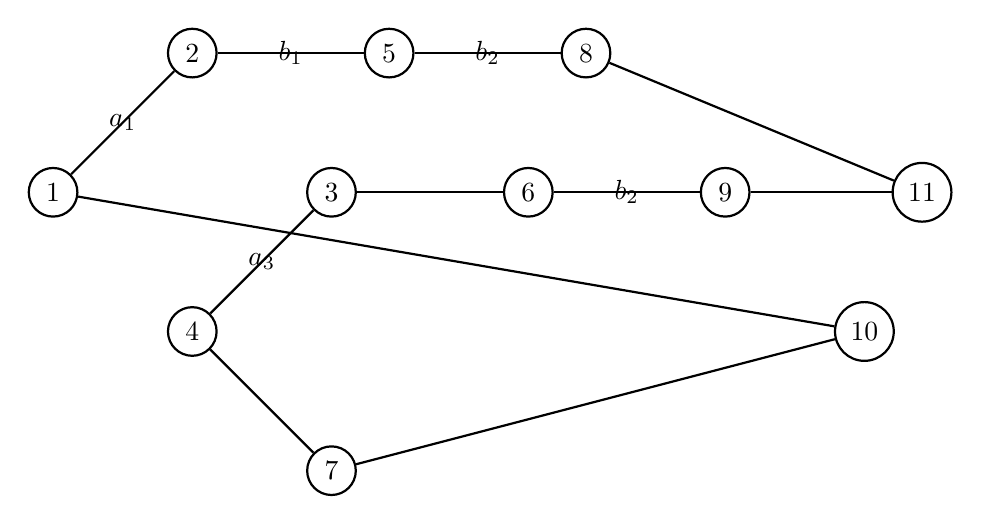
\begin{tikzpicture}[node distance={25mm}, thick, main/.style = {draw, circle}] 
    \node[main] (1) {1};
    \node[main] (2) [above right of=1] {2};
    \node[main] (3) [below right of=2] {3};
    \node[main] (4) [below right of=1] {4};
    \node[main] (5) [right of=2] {5};
    \node[main] (6) [below right of=5] {6};
    \node[main] (7) [below right of=4] {7};
    \node[main] (8) [right of=5] {8};
    \node[main] (9) [below right of=8] {9};
    \node[main] (10) [below right of=9] {10};
    \node[main] (11) [right of=9] {11};

    \draw (1) -- node {$a_1$} (2);
    \draw (2) -- node {$b_1$} (5);
    \draw (5) -- node {$b_2$} (8);
    \draw (8) -- node {} (11);
    \draw (11) -- node {} (9);
    \draw (9) -- node {$b_2$} (6);
    \draw (6) -- node {} (3);
    \draw (3) -- node {$a_3$} (4);
    \draw (4) -- node {} (7);
    \draw (7) -- node {} (10);
    \draw (10) -- node {} (1);
\end{tikzpicture}

\end{document}